\section{Project Methodology}
A software development approach is a structured way of overseeing the creation of a software project. It typically covers aspects such as determining which features to include in the current version, setting release timelines, assigning tasks to team members, and defining the testing process.

\subsection{Software Development Method}
The software development model defines the structured approach used to build the system. Choosing the right model depends on factors such as project size, complexity, and flexibility.

Our project is of medium size with rapidly evolving requirements, requiring a development approach that is adaptable to change. To achieve this, we follow a process that emphasizes collaboration and interaction among team members. The development is structured around short-term plans, which are prepared jointly by the project supervisor and the team. Based on these factors and the comparison shown in Table~\ref{tab:agile}, agile software development methodologies were selected.

\subsection{Agile Software Development Methodologies}
Agile development methodologies are iterative project management approaches that prioritize collaboration, flexibility, and feedback. They break projects into smaller parts, called sprints, with regular reviews and adjustments to allow developers to respond to evolving requirements.

Agile development methodologies are important because they:
\begin{itemize}
    \item Enable faster delivery and quick adaptation to change.
    \item Enhance collaboration among team members and stakeholders.
    \item Increase product relevance through user-centric development.
    \item Reduce cost overruns and improve time to market.
\end{itemize}

A comparison between the most commonly used agile methodologies is shown in the table below.

\renewcommand{\arraystretch}{1.4}

\begin{longtable}{|>{\raggedright\arraybackslash}p{2cm}|>{\raggedright\arraybackslash}p{3.5cm}|>{\raggedright\arraybackslash}p{3.5cm}|>{\raggedright\arraybackslash}p{3.5cm}|}
\hline
\rowcolor{gray!20}
\textbf{Criteria} & \textbf{Scrum} & \textbf{Kanban} & \textbf{Extreme Programming (XP)} \\
\hline
\endfirsthead

\hline
\rowcolor{gray!20}
\textbf{Criteria} & \textbf{Scrum} & \textbf{Kanban} & \textbf{Extreme Programming (XP)} \\
\hline
\endhead

\hline
\multicolumn{4}{r}{\textit{Continued on next page}} \\
\endfoot

\hline
\endlastfoot

Focus & Time-boxed iterations (Sprints) & Continuous flow of work & Engineering practices for quality and responsiveness \\
\hline
Key Roles & Product Owner, Scrum Master, Development Team & No defined roles & Developer, Tester, Customer \\
\hline
Iteration Length & Fixed (2--4 weeks) & Continuous delivery & Short (1--2 weeks) \\
\hline
Work Breakdown & Prioritized backlog & Visualized tasks (Kanban board) & Small features with continuous feedback \\
\hline
Planning & Sprint planning & Pull-based planning & Iterative feature planning \\
\hline
Customer Involvement & High & Moderate & Continuous \\
\hline
Flexibility to Change & Limited during sprint & Highly flexible & Highly flexible \\
\hline
Team Collaboration & Cross-functional teams & Specialized resources & Self-organizing teams \\
\hline

\caption{Comparison among Scrum, XP, and Kanban agile methodologies}
\label{tab:agile}
\end{longtable}

Our project involves a small, cross-functional, and self-organized team with clearly defined roles and fixed deliverables. Based on these characteristics and the comparison above, the Scrum methodology was selected.

\subsection{Scrum Methodology}
Scrum is an Agile framework designed to support effective collaboration in complex software development projects. It emphasizes iterative progress, accountability, and continuous improvement. Work is divided into time-boxed iterations called sprints, typically lasting two to four weeks. Each sprint begins with a planning meeting and ends with a review and retrospective.

\begin{figure}[H]
    \centering
    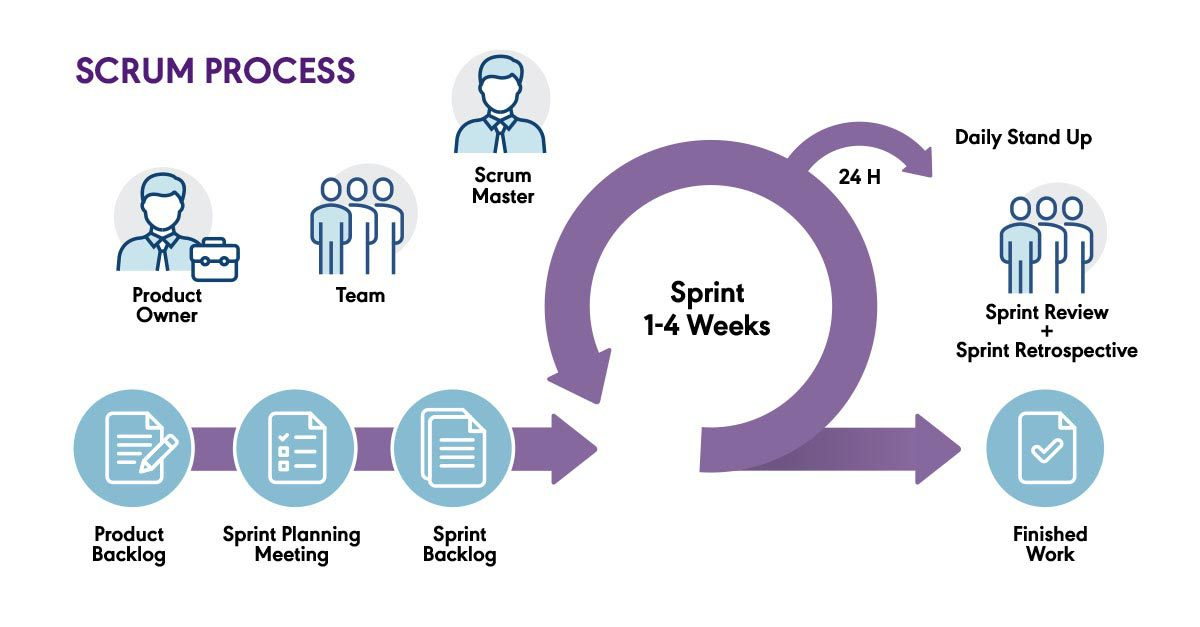
\includegraphics[width=1\linewidth]{images/scrum-process.jpg}
    \caption{Scrum Methodology Process}
    \label{fig:scrum}
\end{figure}

The roles in Scrum are defined as follows:
\begin{itemize}
    \item \textbf{Product Owner (PO):} Responsible for representing stakeholders, defining requirements, and prioritizing the product backlog.
    \item \textbf{Scrum Master:} Ensures adherence to Scrum principles, removes impediments, and facilitates communication within the team.
    \item \textbf{Scrum Team:} A group of professionals responsible for delivering the product increment during each sprint.
\end{itemize}

\subsubsection{The Primary Phases of the Scrum Model}
\begin{enumerate}
    \item \textbf{Initiation:} Defining the project vision, identifying stakeholders, and forming the Scrum team.
    \item \textbf{Planning and Estimation:} Selecting backlog items and planning sprint activities.
    \item \textbf{Implementation:} Executing sprint tasks and updating progress continuously.
    \item \textbf{Reviewing:} Evaluating sprint outcomes and identifying improvements.
    \item \textbf{Releasing:} Delivering the product increment and conducting retrospectives.
\end{enumerate}

\stepcounter{subsubsection}
\subsection{Justification for Technology Choices}

\begin{itemize}
    \item \textbf{Frontend -- Flutter:} Flutter enables a single codebase for web and mobile applications, ensuring faster development, consistent design, and seamless integration with backend services and AI features.
    
    \item \textbf{Backend -- Golang / Spring Boot:} These frameworks provide high performance, scalability, and reliability, making them suitable for handling concurrent requests and multiple database systems.
    
    \item \textbf{Databases -- PostgreSQL and MongoDB:} PostgreSQL manages structured relational data, while MongoDB supports flexible and unstructured data, offering versatility across use cases.
    
    \item \textbf{LLM AI Agent -- AutoGen:} This tool supports natural language interaction, automated schema generation reducing the learning curve for users.

    
    \item \textbf{Cloud Deployment -- AWS / GCP:} Cloud platforms ensure scalability, reliability, secure storage, and flexible deployment while avoiding vendor lock-in.
\end{itemize}

By integrating these technologies, the proposed platform achieves a robust, scalable, and user-friendly environment that enhances productivity and simplifies database management for both novice and experienced developers.
